
\section{Data}\label{section:data}

\subsubsection*{Academies, Scholars, Publications, and Censorship}

Our unit of observation is a scholar active in Italy, to whom we will attach publications and, possibly, censorship. The database is built in three steps.

First, we collect information on all scholars who were appointed to an Italian university or were nominated
to an Italian academy over the period 1450-1750. For universities, the main sources are as follows. An extensive coverage of the University of Bologna is provided by \citeN{mazzetti1847repertorio}. The University of Padova is covered by \citeN{facciolati1757fasti}: we complete its information with the works by \citeN{casellato2002professori}  and \citeN{pesenti1984professori}. Professors at the university in Rome, Sapienza, were found in \citeN{renazzi1803storia}. The professors at University of Naples are covered by \citeN{paolino1754istoria}. Pavia is another well-documented university:  \citeN{raggi1879memorie} lists all its professors. Pisa is covered in \citeN{fabroni1795historiae}. The smaller University of Macerata also benefits from a full coverage by \citeN{serangeli2010docenti}.
For academies, we use the database ``Italian Academies 1525-1700, the first intellectual networks of early modern Europe'' made available by the British Library in 2013. Among the academies covered, the Gelati and the Ricovrati are two important ones. We complete these data with \citeN{parodi1983catalogo} for the language academy ``La Crusca'' and with \citeN{maggiolo1983soci} for a full coverage of the biggest academy, the Ricovrati. In appendices \ref{O-appendix:data2} and \ref{O-appendix:data1}  we discuss how representative  data are, and how much of the Italian university/academy population is covered.
Figure~\ref{O-fig:dempster} in Appendix~\ref{O-appendix:dempster} shows an example. Tommaso Dempstero is in the list compiled by \citeN{mazzetti1847repertorio} of professors at the University of Bologna. We also find him in the history of the University of Pisa by \citeN{fabroni1795historiae}, under his Latin name, Thomas Dempsterus. Checking the Italian encyclopedia from the  \citeN{treccani1929Enciclopedia}, we corroborate the information on Bologna.

Second, we use the Worldcat search engine, which provides references to the collections of thousands of libraries around the world, to assign to each scholar all the written output he/she generated, including post mortem editions.  More precisely, we count the number of ``publications'', including different editions of the same work. We only record publications by the author, and exclude publications about the author. Worldcat provides a good approximation of the population of known European authors.
\citeN{chaney2020}  compares the Universal Short Title Catalogue \cite{USTC} to the references in the Virtual International Authority File (VIAF), on which WorldCat is based. Chaney successfully locates 81\% of USTC authors in the VIAF.
Figure~\ref{O-fig:dempster} shows the Worldcat Page for Thomas Dempster, with the total count of publications (by or about). We can identify the two types of publications by scraping the page. From the graph on the webpage, we can see that all publications are by him.
In a third step, we look at the list of forbidden books from \citeN{de2002index} and \citeN{de1996thesaurus}. We find an entry for Thomas Dempster with a short biography and the list of books that were forbidden, with the date of the corresponding decrees.


We now show some statistics on the number of scholars and on their publications. In Table~\ref{tab:publi} the period 1400-1750 has been divided into five periods of 70 years each.
The first line covers all of Europe, from the database built by \citeN{RETE}, and includes both universities and academies. Columns (1) to (5) contain the number of ``published'' scholars per period, i.e. those having some work referenced in Worldcat.  Columns (6) to (10) show the median number of publications per person. The second line covers the subset of scholars affiliated to an Italian institution.

%UPDATED 29 AUG 2022=========================================================================================================================
\begin{table}[!htbp]
\centering
		\begin{tabular}{@{ \extracolsep{3pt}}lcccccccccc}%x}{\textwidth}{l *{10}{Y}}
\toprule
			& \multicolumn{5}{c}{Total number of }  & \multicolumn{5}{c}{Median number of }\\
			& \multicolumn{5}{c}{published scholars}  & \multicolumn{5}{c}{ publications per person}\\
			Period   & 1 &2 & 3 & 4 & 5  & 1 &2 & 3 & 4 & 5\\
\midrule
Europe                   & 416      & 1294     & 2892     & 3756     & 5495     & 28       & 55       & 63       & 59       & 52 \\
Italy                    & 210      & 402      & 764      & 758      & 779      & 72       & 95       & 73       & 40       & 28 \\
France                   & 54       & 209      & 488      & 729      & 943      & 20       & 86       & 87       & 63       & 61 \\
Germany \& Austria       & 84       & 466      & 968      & 989      & 2056     & 9        & 52       & 67       & 122      & 97 \\
Great Britain \& Ireland & 15       & 57       & 162      & 356      & 920      & 15       & 77       & 149      & 218      & 145 \\
Denmark \& Sweden        & 1        & 13       & 55       & 146      & 338      & 5        & 25       & 62       & 60       & 82 \\
Spain \& Portugal        & 25       & 97       & 263      & 210      & 192      & 32       & 50       & 33       & 15       & 6 \\
\bottomrule
			\multicolumn{11}{l}{\footnotesize Note: periods: 1:1400-69, 2:1470-1539, 3:1540-1609, 4:1610-79, 5:1680-1749}
	\end{tabular}
	\caption{Total number of scholars \& publications by period}\label{tab:publi}
\end{table}


The number of publications per person illustrates the decline of Italy. It is both a relative decline (relative to the rest of Europe), and an absolute decline. Until period 2 (1470-1540), published scholars in Italy produced an output higher than the average European scholar. Then, a reversal appears in period 3 (1540-1610) and the gap becomes  wide in period 5 (1680-1750). The appearance of the gap coincides with the
formalization of censorship through the first index published by the University of Paris in 1544, and the first Roman Index, also known as the {\em Pauline Index}, promulgated by Pope Paul IV in 1559 \cite{de2002index}. Note that the Catholic Church also censored scholars who never visited Italy, but the Church struggled to enforce censorship outside Italy \cite{putnam1906}.\footnote{\citeN{putnam1906} notes that also the other European States created and enforced their indexes and controlled the press. He also notes that these restrictions were generally less well-enforced than the Roman indexes and bore less serious consequences for the production of knowledge, except for Spain where censorship has been carried on with consistency and thoroughness. The Roman censorship also found some difficulties in being enforced in Italy outside the Papal State, but recent estimates by \citeN{becker2021} suggest that it has been applied more widely than previously thought. }
In Appendix~\ref{O-app:robustdecline}, we show that the decline of Italy we highlighted is robust to the way it is measured. The same pattern is observed using the number of scholars per inhabitant, other measures of publications, and Wikipedia pages.

Table~\ref{tab:publi} also shows statistics for  individual countries. %\footnote{We did not show the results for all European countries because some have too few observations or contained scholars coming from one University/academy only (this is the case of Belgium and the University of Louvain).}
 For countries like France, Germany and Austria we can observe that until period 2 (1470-1540) published scholars produce a similar or lower output than Italy, while a gap appears in the following periods. Note that eventually these countries reach a level of output unknown to Italy. A similar pattern can be observed for Great Britain, Ireland, Denmark, and Sweden, with the caveat that we have very few observations for these countries in the first two periods. The case of Spain and Portugal is different, as these countries do not overtake Italy. This is not surprising given the intensity of the Spanish Inquisition \cite{vidal2011}.


Table~\ref{O-tab:publiIT} in Appendix \ref{O-app:pub-by-instit} disaggregates the Italian numbers by (important) institutions. The decline from period 3 to period 5 is present in the universities of Bologna, Padua,  Pavia,  Pisa, Torino, in the two Roman universities, and in the Florentine Studium. The academies do better, in particular the Ricovrati, but this is not enough to compensate for the overall decline at the Italian level.



One can argue that the decline in knowledge production in Italy might be because the standard required to become a professional scholar declined. In fact, if published scholars are positively selected and the barriers to entry weaken, the median quality of scholars goes down. One way to control for this problem is to look at the dynamics of top scholars, who are less affected by changes in the barriers to entry. Hence, in Table~\ref{O-table:europewiki} in the appendix, we show that Italy still loses to Europe in terms of knowledge production if we consider only scholars whose longest Wikipedia page (across all languages) is longer than 5000 characters. Moreover, in Appendix~\ref{O-appendix:data3} we show that Italy is overtaken by Europe within all the scholars' fields that we are able to identify, ruling out the possibility that the this observation was driven by a composition effect across fields.




\subsubsection*{Two Features of Author Censorship}\label{section:twof}

On May 23 1555, a new Pope was elected and Cardinal Caraffa became Paul IV. This election heralded the return of the conservatives. In 1559, Paul IV had published the first long list of prohibited books, the Index. The idea was refined further by the Council of Trent, which established in 1564 the \textit{Index Librorum Prohibitorum}. The Index comprised three parts. The first part contained the name of the heretical authors whose entire output, past and future, was condemned (\textit{opera omnia}, all the works). The second part contained a list of censored publications by authors who still belonged to the Church. The third part dealt with anonymous publications.

This attempt to control publications by the Catholic Church is probably the biggest experiment in the history of censorship.\footnote{Earlier prohibitions were limited in scope and only affected the immediate locality in which the prohibition was issued \cite{putnam1906}.} The entirety of ideas accessible to citizens had to be controlled to maintain the predominance of the Church. The Inquisition was responsible for the enforcement of censorship: the punishments for reading and keeping censored books included excommunication, eternal damnation, and confiscation of assets, which helped finance the inquisitory apparatus \cite{maifreda2014denari}. Censorship lasted four centuries, as the last version of the Index was published in 1948.



The Index was established following a change in the attitude of the Church towards novel ideas, including scientific ones. The Copernicus case best illustrates the reversal of attitude. The idea of his heliocentric system was developed around 1505, and first documented in an unpublished book intended for his friends. The Pope Clement VII learned about these ideas in 1533 and liked them. Several highly ranked clerics asked Copernicus to publish his treaty. One advantage of Copernicus's system was to provide more accurate computations for astronomical events. Then, after the conservative revolution, Copernicus's writings were blacklisted. What appeared to be a legitimate hypothesis in 1543 became in 1616 a foolish thesis, absurd in philosophy, and formally heretic. The Church took more than three centuries to accept heliocentrism and removed Copernicus's works from the Index in 1846.

The Church's fight did not spare the most notable forerunners of the varied flow of novel ideas that spread all over Italy and Europe. Galileo Galilei was condemned, and his books were censored not only for his astronomical views, but also for his support of atomism. According to atomism, the physical world comprises fundamental, indivisible components known as atoms, violating the Aristotelian view of a continuous matter. Atomism and its proponents, such as the French philosopher Descartes, were censored by the Church until at least the beginning of the eighteenth century. In a world where religion and philosophy were intertwined with natural sciences, the aversion towards atomism is likely to have affected scientific knowledge. Perhaps it is not a coincidence that the particle theory of light, which relies on an atomist view of the matter, was developed by Newton and not by an Italian.

The Church's fight had some consequences for thinking about the continuum,  indivisibles, and the actual infinite. The Jesuits were particularly active in these mathematical controversies, fighting against the idea that a continuous line is composed of distinct and infinitely tiny parts  \cite{alexander2014infinitesimal}.
In his book, \citeN{alexander2014infinitesimal} considers what the world would have been like without infinitesimals. ``If the Jesuits and their allies had had their way, there would be no calculus, no analysis, nor any of the scientific and technological innovations that flowed from these powerful mathematical techniques.''
Now, this is perhaps exaggerated, and Alexander claims more than he is able to prove. \citeN{grabiner14} defends the view that seventeenth-century mathematics had far too much momentum and too many demonstrable successes to be stopped by philosophical arguments about the nature of the continuum.

Another landmark of the reversal in the attitude of the Church is the censorship of all the works by, and the burning at the stake of Giordano Bruno.
Bruno had accumulated many reasons to be condemned to death, but one point of his theory that did not fit at all with the Church's view was the theoretical possibility of an infinite universe and a plurality of worlds. Bruno has become the symbol of the scientist persecuted by religious authorities. In other times authors were punished with imprisonment: a notable example is Galilei.

Looking at the data in the \textit{Index Librorum Prohibitorum}, one should admit that censorship does not necessarily imply that the author risks his life. While sometimes, as for Bruno and Galilei, censorship went together with severe consequences for the author; in other cases, the consequences were mild. For example, the poet John Barclay, whose works contained satirical descriptions of the Jesuit school, was listed in the Index in 1608.  At the invitation of the Pope himself, he went to Rome in 1616 and resided there until he died in 1621. Moving to Rome was a way to signal that he was a good Catholic and avoid further consequences. Not all of his writings were blacklisted, and he was able to publish again after he was first censored. In other cases, there were no consequences for the author simply because the heresy was identified after her/his death. This is the case of Bernardino Ciaffoni, who %used to be the rector of Rome's college San Bonaventura. He
died in 1684 but was censored in 1701 because his works contained insulting claims against the Jesuits. Scholars developed different strategies to avoid negative repercussions from their writings. In sum, censorship did not always bring negative consequences for the authors, while posterity paid a premium for complicated access to the revolutionaries' wisdom, at least that embodied in forbidden books.


Being a clergyman did not confer protection against censorship. One particularly striking case is Serry Jacobus Hyacinthus. A Professor in Padova, he contributed to the Dominicans-Jesuits controversy on grace, and several of his works appeared in the Index. Not only he was a Dominican, but also he was a member of the \textit{Congregation of the Index}, the body responsible for the creation and management of the Index. Censorship did not spare even the members of the company of Jesus, who had a primary role in the Counter-Reformation. In our database, 10 out of 173 published scholars belonging to the Jesuit university Gregoriana were censored. %Among them, Achille Gagliardi was censored in 1703 for his writings about the annihilation of the will during mystical states. These ideas were found to be incompatible with free will, which is a cornerstone of Catholic theology.

We now describe  censorship quantitatively. Figure~\ref{fig:distrib} shows how authors belonging to our dataset are distributed according to the number of their publications. We mark authors who were censored at least once in red, and non-censored authors in green. We provide five histograms, one for each period. Censorship started at the end of the second period, but also affected works that were published in the past. From these five histograms, it is clear that censorship was concentrated on top scholars for the first two to three periods, and then became more uniformly distributed over the quality of scholars. Or, as we wrote earlier, once censorship was introduced, censored authors were of better quality than the non-censored authors, but this gap shrank over time. For an alternative visualization of the changing gap in quality between censored and non-censored authors, see Figure~\ref{O-fig:alter} in Appendix~\ref{O-app:prf4}.

This shift in the identity of who was impacted by censorship reflects behavioral changes. The top scholars who had the potential to publish non-compliant ideas and become famous (as in the first three periods) decided to be more compliant, and published conventional material instead. Bruno, Copernicus and Galilei were at the top of the distribution and were all censored, and sometimes burned. Their similarly talented successors in the last two periods might have been published as mediocre poets.

%UPDATED 29 AUG 2022=========================================================================================================================
%%Table with moments to be fit%%
\begin{table}[htbp]
	\centering
\begin{tabularx}{\textwidth}{ l *{5}{Y}}
\toprule
Moment description& \multicolumn{5}{c}{Period}\\
   & 1400-69 &1470-1539 & 1540-1609 & 1610-79 & 1680-1749 \\
\midrule
Number of published scholars (all)
    &  210 &  402 & 764 & 758 & 779 \\
\% censored scholars
    & 6.67 &10.95 &7.85 &6.60 & 4.49 \\
    \\
Log publications per scholar (all), median (1)
    & 4.27 &4.55 & 4.29 &3.68 &3.33 \\
Log publications per  scholar (censored), median (2)
    &  7.73 &7.07 & 7.07 &5.67 &5.87  \\
Gap in median publications (2)-(1)
    &  3.46     &  2.52      &  2.78     &  1.99    &  2.55  \\
    \\
Log publications per scholar (all), $75^{th}$ percentile
    &  5.73& 5.98 & 5.56 &5.05 &5.16 \\
Log publications per scholar (censored), $75^{th}$ pctl
    & 7.89 &7.91 & 8.16 &7.27 &6.81  \\
\bottomrule
\end{tabularx}
\caption{Moments per period}\label{table:momentstofit}
\end{table}


%=============================================================================
%                   starting date                    1400 1470  1540 1610 1680
%                     end date                       1470 1540  1610 1680 1750
%        Number of published scholars (all)          210   402  764  758  779
%    Log publications per scholar (all), median      4.27 4.55  4.29 3.68 3.33
%  Log publications per scholar (censored), median   7.73 7.07  7.07 5.67 5.87
%  Log publications per scholar (all), 75th perc.    5.73 5.98  5.56 5.05 5.16
%Log publications per scholar (censored), 75th perc. 7.89 7.91  8.16 7.27 6.81
%                % censored scholars                 6.67 10.95 7.85 6.6  4.49
%----------------------------------------------------------------------------- 


%UPDATED 29 AUG 2022=========================================================================================================================
\begin{figure}[p]
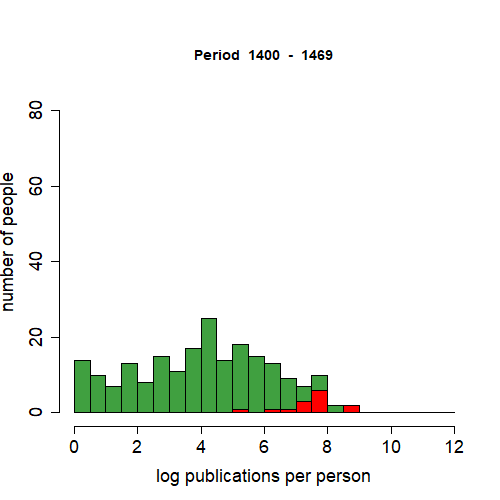
\includegraphics[width=.33\textwidth,trim=0cm 0cm 0cm 1.5cm, clip]{histo1Q.png}
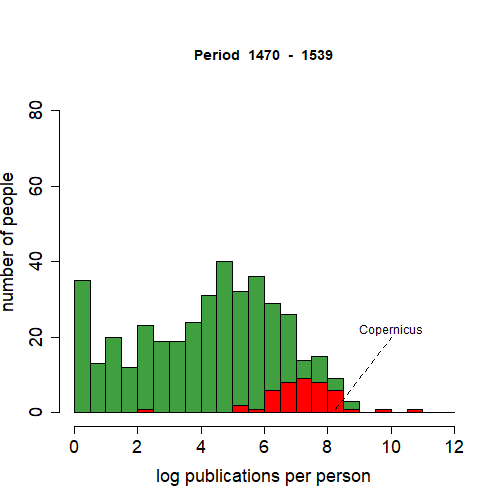
\includegraphics[width=.33\textwidth,trim=0cm 0cm 0cm 1.5cm, clip]{histo2Q.png}

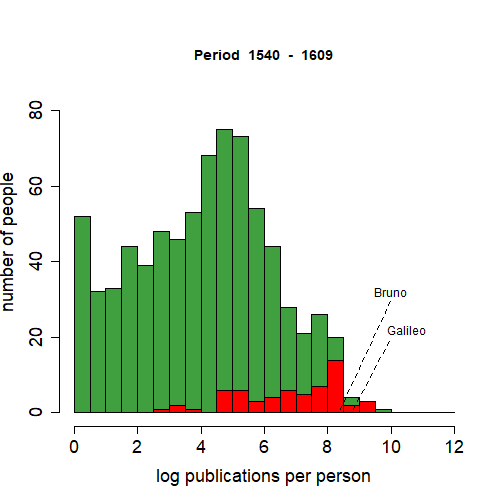
\includegraphics[width=.32\textwidth,trim=0cm 0cm 0cm 1cm, clip]{histo3Q.png}
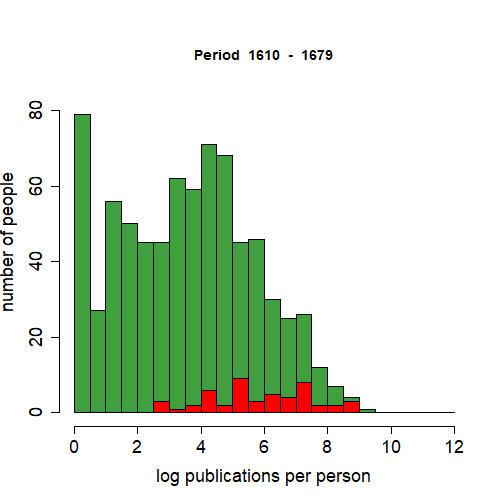
\includegraphics[width=.32\textwidth,trim=0cm 0cm 0cm 1cm, clip]{histo4Q.png}
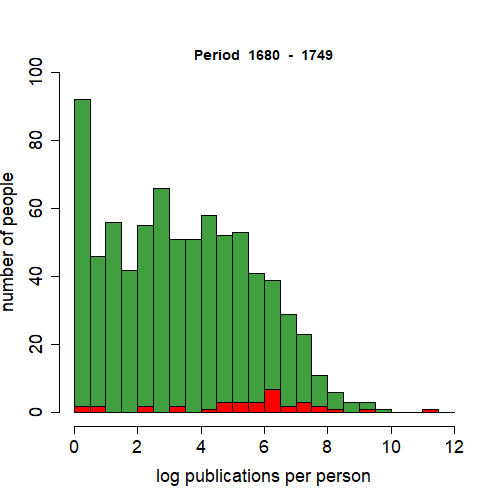
\includegraphics[width=.32\textwidth,trim=0cm 0cm 0cm 1cm, clip]{histo5Q.png}

\caption{Distribution of published authors by quality. Red: censored. Green: non-censored. }\label{fig:distrib}

\end{figure}

%UPDATED 29 AUG 2022=========================================================================================================================
\begin{figure}[p]
\begin{center}
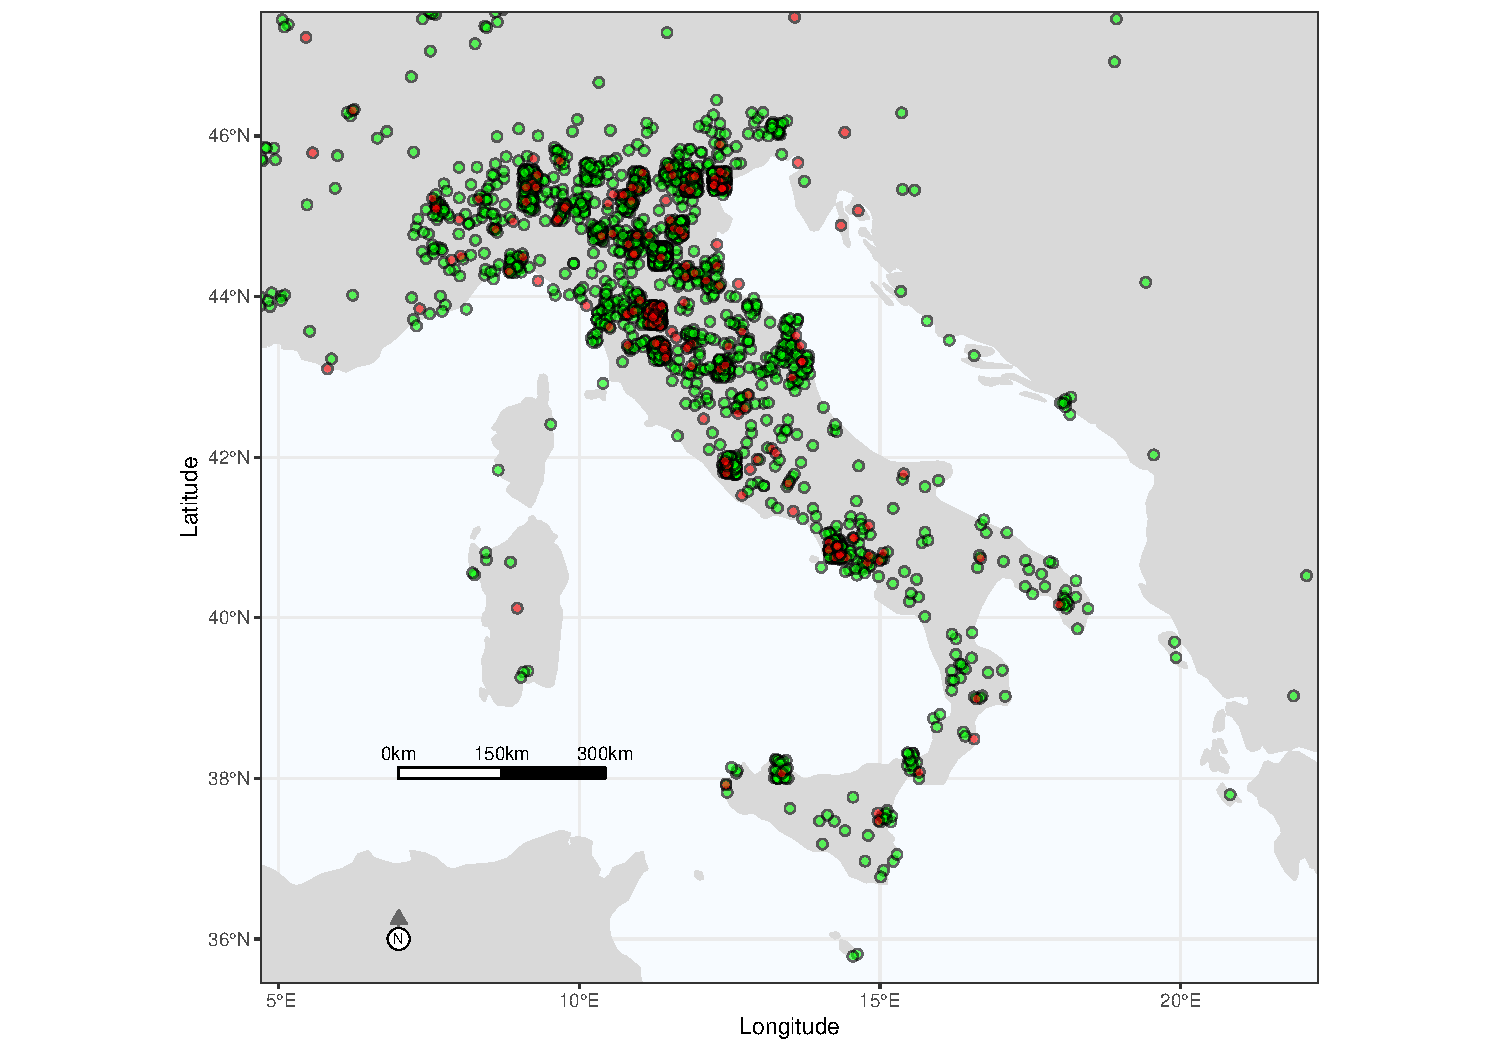
\includegraphics[width=.57\textwidth,trim=3cm 0cm 3cm 0cm,clip]{map-italy.pdf}
\end{center}
\caption{Place of birth of censored (red) and non censored (green) members of Italian universities \& academies -- Italy. }\label{fig:italy}
\end{figure}

We show in Table~\ref{table:momentstofit} the key moments of these distributions. It confirms what we expected from the figures: the gap in median publications between censored authors and all authors shrank from about 3.4 to 2.4 (the numbers should be interpreted as log of number of publications).  The table shows two additional features. First, after the second period, the percentage of censored authors is shrinking over time. Second, overall quality, measured by median publications per person, is declining over time as well. This also holds for the top of the distribution, as the 75th percentile also diminishes over the last four periods. Those two trends are very much compatible with the idea of the top innovators' books becoming progressively compliant and of lower quality over time.




Our data also reveals possible geographical patterns in censorship. Figure~\ref{fig:italy} shows the place of birth of the scholars in the database, distinguishing the censored (red) from the not censored (green) ones. Geographical coordinates have been slightly randomized, so that people born in cities still appear distinctly. From the map of Italy, we can observe that our data cover the whole peninsula and its islands. Moreover, censorship  affects all regions rather uniformly.



Some members of Italian universities and academies were born outside Italy (as with Thomas Dempster in our example above). Hence the interest in having a map of Europe. Figure~\ref{O-fig:europe} in Appendix~\ref{O-fig:europe} provides a European view of the places of birth of our scholars. Some of them are foreign or corresponding members of some academies, such as the Ricovrati. They might have never come to Italy, so we use a specific robustness test that excludes those foreigners.





